\documentclass[12pt,a4paper,utf8x]{report}
\usepackage [frenchb]{babel}
\usepackage[utf8]{inputenc}  
\usepackage[T1]{fontenc} 
% Pour pouvoir utiliser 
\usepackage{ucs}

\usepackage{textcomp}
\usepackage{graphicx}
\usepackage{keystroke}
\usepackage{amssymb}
\usepackage{amsmath}
%\usepackage{pifont}

\usepackage{url} % Pour avoir de belles url
\usepackage{geometry}
\usepackage{hyperref}
%[linktocpage]
% Pour mettre du code source
\usepackage {listings}
\lstset{language=sh}

% Pour pouvoir passer en paysage
\usepackage{lscape}

% Pour pouvoir faire plusieurs colonnes
\usepackage {multicol}
% POur crééer un index
\usepackage{makeidx}
\usepackage{graphicx}
\usepackage{tocbibind}
\hypersetup{
backref=true,
%permet d'ajouter des liens dans...
pagebackref=true,%...les bibliographies
hyperindex=true, %ajoute des liens dans les index.
colorlinks=true, %colorise les liens
breaklinks=true, %permet le retour à la ligne dans les liens trop longs
urlcolor= blue, %couleur des hyperliens
linkcolor= blue, %couleur des liens internes
bookmarks=true, %créé des signets pour Acrobat
bookmarksopen=true,
%si les signets Acrobat sont créés,
%les afficher complètement.
pdftitle={Manuel Utilisateur pour LoCD}, %informations apparaissant dans
pdfauthor={MARGUERITE Alain\\ RINCE Romain},
%dans les informations du document
pdfsubject={LoCD}
%sous Acrobat.
}
%pied de page
\usepackage{fancyhdr}
\pagestyle{fancy}
\fancyhf{}
\fancypagestyle{plain}{
\fancyfoot[C]{\thepage}
\fancyhead[C]{\leftmark} 
 %\renewcommand{\headrulewidth}{0pt} % ...et le filet
}
%\renewcommand{\headrulewidth}{0.5pt}  %trait horizontal en tête
\renewcommand{\footrulewidth}{0.5pt} %trait horizontal pied de page

%\renewcommand{\chaptermark}[1]{\markboth{#1}{}}
\renewcommand{\sectionmark}[1]{\markright{#1}}

%\renewcommand{\footrulewidth}{0.5pt}

\renewcommand{\labelitemi}{$\bullet$}%changer les puces 
\makeindex


%%%% debut macro pour enlever le nom chapitre %%%%
\makeatletter
\def\@makechapterhead#1{%
  \vspace*{50\p@}%
  {\parindent \z@ \raggedright \normalfont
    \interlinepenalty\@M
    \ifnum \c@secnumdepth >\m@ne
        \Huge\bfseries \thechapter\quad
    \fi
    \Huge \bfseries #1\par\nobreak
    \vskip 40\p@
  }}

\def\@makeschapterhead#1{%
  \vspace*{50\p@}%
  {\parindent \z@ \raggedright
    \normalfont
    \interlinepenalty\@M
    \Huge \bfseries  #1\par\nobreak
    \vskip 40\p@
  }}
\makeatother
%%%% fin macro %%%%



%Couverture 


\title
{Manuel Utilisateur pour LoCD}



\author{MARGUERITE Alain\\ RINCE Romain}

\date{Université de Nantes \\ 2 rue de la Houssinière, BP92208, F-44322 Nantes cedex 03, FRANCE}

\begin{document}

\maketitle


\clearpage

\tableofcontents
\clearpage

% Pour avoir un interligne de 1,5
%\chapter{Étude des structures de données}


%nombre de caractéristiques ?? de quels type 

%Regarder JDK allocation d'une boite structure


%lister toutes les possibilité - garder toutes les structures - reconstruire l'arbre.. refaire une passe sur le fichier


\section{Introduction}
L'objectif de ce document est de mener une étude sur les différentes structures de données nécessaires aux futurs algorithmes de visualisation. Nous nous intéresserons en particulier à l'opération d'accès à une caractéristique ou d'une donnée d'une boîte ainsi qu'à l'occupation mémoire de cette dernière. Il s'appuie sur le document de spécification (cf : annexe). Ce document sur les calculs de complexité seront réalisés selon le paramètre $n$  représentant le nombre de boîtes, et $d$ est le nombre de dimensions du problème. Le nombre de boîtes réellement utilisées dans le pavage est représenté par $N$. 


\section{Définition de la boîte}
C'est l'entité atomique du pavage. Les accès à ses attributs sont donc cruciaux. On rappelle qu'une boîte est définie de la manière suivante : 
\begin{itemize}
\item 
  Un identifiant : soit des chaînes de caractères (IDStr) respectant un format précis (c.f 1.1 du document de spécifications), soit des entiers positifs (IDInt).
\item
  Une liste de coordonnées dans l'ordre des variables définies en entête. Une liste de type \verb+Interval+.
\item
  Une liste des caractéristiques, dans l'ordre et selon les types définis en entête.
\end{itemize}
Ces données seront régulièrement requises lors de la mise en œuvre des algorithmes nécessaires à la visualisation. Il est donc important que leurs accès soient rapides, voire directs. Pour le cas de l'identifiant, s'agissant d'une simple \verb+String+ le problème de la structure à utiliser ne se pose pas. Pour la liste des coordonnées en revanche, il s'agit d'une séquence finie de données. Plusieurs possibilités sont alors envisageables : 

\begin{itemize}
\item
  Un tableau : L'accès à une coordonnée est direct. Les opérations d'ajout et de suppression sont en revanches coûteuses pour les tableaux dynamiques ($O(n)$).
\item
  Une liste : Si l'accès à une coordonnée n'est pas direct ($O(n)$), les opérations d'ajout et de suppression sont en temps constant.
\item
  Une table de hachage : Coûteuse si la fonction de hachage n'est pas appropriée, une table de hachage propose cependant un accès en $O(1)$.  Cependant le phénomène de collisions (mauvaise répartition des clefs entrainant un conflit entre deux valeurs) est à prendre en considération :

\begin{description}
\item[Implémentation avec un tableau dynamique] Une telle structure permet de garantir un accès en temps constant. Cependant chaque collision va doubler l'occupation mémoire du tableau. Or même si la fonction de hachage est bonne, il est possible d'avoir au moins une collision, ce qui aurait pour conséquence une perte de l'espace mémoire qui se répercuterait sur chaque boîte.
\item[Gestion des collisions avec chaînage] Contrairement à la structure précédente, cette méthode permet de ne pas occuper trop d'espace en chainant les éléments entrants en collision. Malheureusement la complexité en pire cas des opérations d'accès passe en $O(n)$. En revanche, grâce à une bonne fonction de hachage, on accèdera généralement en temps constant sans contre coût mémoire. 
\end{description}

Le passage en revue de ces différentes structures écarte la liste et la table de hachage implémentée par un tableau dynamique. En effet les performances des opérations d'accès de la liste ne sont pas raisonnables. De même l'implémentation d'une table de hachage par un tableau dynamique risque d'entrainer une perte de mémoire trop importante.
%\item
 % Une TreeMap \cite{TreeMap}. Implémentation de base des arbres rouges noirs, cette map a la particularité de posséder des clefs triées. Ainsi les complexités de plusieurs opérations telle que l'accès en $O(\log{n})$. Dans le cas d'un grand nombre de valeurs à stocker, il est plus performant de construire la TreeMap à partir d'une HashMap.

\end{itemize}

%La création d'une boîte a alors une complexité en $O(d)$. De plus l'accès aux différents attributs de la boîte (identifiant, liste des coordonnées) sera en $O(1)$.

\subsection{Généricité des caractéristiques}
Un problème majeur apparaît pour l'instanciation des boîtes. On rappelle qu'une caractéristique à plusieurs types (\verb+String+, \verb+Number+ ou \verb+Interval+). Plusieurs solutions sont envisageables : 
\begin{itemize}
\item
  Une Map unique contenant des \verb+String+ stocke les différentes caractéristiques de la boîte. On aura casté les attributs \verb+Number+ ou \verb+Interval+ en \verb+String+. Il sera alors nécessaire, pour chaque futurs accès, d'effectuer un cast dynamique. On rajoute alors une constante supplémentaire à la complexité de cette opération. 
\item 
Trois tableaux (un pour chaque type) au sein d'une boîte. Trois Maps (une pour chaque type) «générales» au niveau du pavage. La clef d'une map est l'id de la caractéristique et la valeur de la map son indice dans le tableau concret. La boîte peut alors retrouver la valeur de la caractéristique au sein de son tableau.
\item 
  Chaque boîte possède trois Maps pour ces trois types de caractéristiques. 
\end{itemize}


\section{Pavage}
\subsection{Problématique}
%L'outil de visualisation peut charger un fichier entrée de manière dynamique ou non. Nous nous plaçons ici dans le cadre où cette option de chargement dynamique n'est pas activée. \\ 
%L'outil va lire séquentiellement chaque ligne du fichier d'entrée.
Le cahier de spécification exige de l'outil la capacité à charger un pavage de taille non déterminée. Si le nombre de boîtes sera en pratique necessairement borné (limite mémoire de la machine), il faut cependant répondre à cette attente en proposant une structure de stockage capable de supporter un très grand nombre de boîtes. De plus l'outil doit être en mesure de fournir régulièrement des listing spéfiques de boîtes. Par exemple pour afficher la liste de celles concernées par un filtre. La structure du pavage doit être en mesure de répondre de manière efficace à des requêtes de séquences de boîtes selon un ordre particulier. La structure du pavage doit être aussi en mesure de répondre efficacement à la structure  de visualisation graphique (founir rapidement les nouvelles boîtes dans le champs de visualisation, lors d'une rotation de caméra par exemple). Quelles structures de données et quelles stratégies choisir face à de telles exigences ?  %Ce chapitre débute par de le passage en revue de différentes structures de données potentielles. % La création de la structure de stockage débute par la lecture séquentielle du fichier d'entrée (cf section 1  du document de spécification). Plusieurs options apparaissent à cette étape, faut-il par exemple :


%  Le fichier d'entrée est lu une unique fois. Les méthodes de structures dans laquelle les boîtes sont stockées sont suffisamment performantes pour répondre à toutes les spécifications. On peut alors se poser la question s'il faut :


%\begin{enumerate}
 % \item
 %   Insérer les boîtes dans la structure puis la trier plus tard ?
 % \item
 %   Utiliser un tri par insertion ?
%\end{enumerate}


 % Il est possible que refaire des «passes» sur le fichier d'entrée soit une solution. Dans les cas où les opérations de tris et/ou de recherches seraient trop coûteuses pour la structure du pavage (par exemple lors d'une demande de listing de certaines boîtes). On aurait une complexité en pire cas en $O(n)$. 
  % Le création de structure de  données peut alors se faire de différentes  manières : 

\subsection{\'Etude de structures}

\paragraph{Vector :} Collection de données à accès direct par indice. Le nombre de boîte étant donné dans l'entête du fichier d'entrée, une implémenation par un tableau statique proposerait une complexité en $O(n)$ pour l'opération de stockage du pavage. Si l'accès à une boîte à partir de son indice serait direct, l'opération de recherche en revanche aurait une complexité en $O(n)$. 

\paragraph{Dictionnaire :} Collection de données à accès direct par clef. Dans l'hypothèse de posséder une fonction de hachage ne provoquant pas de collisions, une implémentation par une fonction de hachage propose une complexité en $O(n)$ (à nouveau grâce à la connaissance du nombre de boîtes dans l'entête du fichier d'entrée).


%Le nombre potentiellement très grand de boîtes élimine d'emblée la possibilité de choisir une HashMap. En effet même si la fonction de hashage est judicieusement choisie, l'occupation mémoire requise serait bien trop importante. Les listes ne sont pas  appropriées ici. Une complexité en $O(n²)$ pour un accès à une boîte n'est pas raisonnable. Les arbres ont l'atout de pouvoir stocker et manipuler un grand nombre de d'entités. Les arbres de recherches sont des arborescences ordonnées permettant un accès en $O(\log(n))$. Dans le cas où la structure serait triée au fur et à mesure de sa construction. Les arbres de recherche proposent de bonnes performances. Nous développerons pourquoi à travers des cas d'exemples dans les prochains paragraphes : 


\paragraph{Arbre binaire}
Par exemple l'utilisation d'un arbre binaire de recherche pour la création de n boîtes aurait une complexité de $n²$ en pire cas. En effet il s'agit du cas où les boîtes arriveraient triées selon l'ordre inverse de celui que l'on souhaite. Il faudrait alors effectuer $(p-1)$ comparaisons, pour chaque boîte :  $\sum_{p=2}^{n}(p-1)$  Soit $O(n)=\frac{1}{2}n²-\frac{1}{2}n$. Cependant dans le meilleur des cas cette opération a une complexité en $O(n\log{n})$. La création d'un pavage composé de $n$ boîtes à $d$ dimensions aurait alors une complexité égale à: $O(d \times n\log(n))$ 

\begin{figure}[htbp]
  \centering
  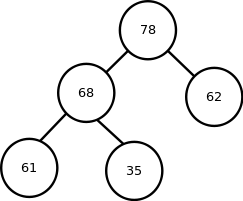
\includegraphics[scale=0.60]{img/binTree}
  \caption{arbre binaire}
  \label{fig:abtree}
\end{figure}
L'arbre binaire était équilibré par définition, la compléxité de son opération de recherche est en $O(log_2 n)$ (hauteur de l'arbre).
   


%http://www.enseignement.polytechnique.fr/profs/informatique/Luc.Maranget/421/poly/arbre-bin.html
\clearpage
\paragraph{Arbres a-b}
Il s'agit d'un arbre de recherche avec les propriétés suivantes :
\begin{itemize}
\item
  $a\leq2$ et $b\leq 2a−1$ deux entiers.
\item
  La racine a au moins 2 fils (sauf si l'arbre ne possède qu'un nœud) et au plus b fils.
  Les feuilles sont de même profondeur.
\item
  Les autres nœuds internes ont au moins a et au plus b fils.
\end{itemize}

\begin{figure}[htbp]
  \centering
  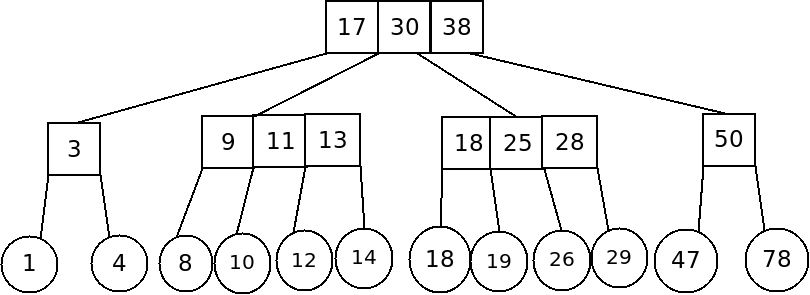
\includegraphics[scale=0.40]{img/abtree}
  \caption{a-b arbre}
  \label{fig:abtree}
\end{figure}

L'avantage des arbres a-b est que leurs hauteurs  sont comprises entres les valeurs suivantes : $ \dfrac{\log{n}}{\log{b}}   \leq h  < 1 + \dfrac{\log{n/2}}{\log{a}}$. Ainsi les opérations d'insertion ne seraient plus en $O(n\log{n})$ mais en $O(\log{n})$. La création d'un pavage composé de $n$ boîtes à $d$ dimensions aurait alors une complexité en $O((n\times d)\log(n))$. La recherche d'un boîte quant à elle aurait une compléxité en $O(\log{n})$.


\section{Introduction et objectifs}
\label{chap:fichDonnees}
\subsection{Avis au lecteur} 
Ce manuel est destiné à un public désirant utiliser le logiciel GT. C'est à dire depuis son installation jusqu'à la génération du fichier au d'un fichier au format .ktr.Le manuel n'a pas pour objectif d'enseigner l'utilisation de cet outil. Les auteurs recommandes l'ouvrage suivant pour un tel apprentissage : \cite{kiwi}.

\subsection{Présentation du logiciel GT}
GT permet la génération automatique ou manuel de de systèmes temps réel.  L'outil est dédié est uniquement utilisable en mode console.

\section{Installation et configuration}

\subsection{Configuration nécessaire}
\label{sec:conf}
\index{Configuration requise}
\danger : GT est un outil open source dédié uniquement aux systèmes d'exploitation linux. Il n'existe pas encore de version pour Windows et MAC OS. L'installation requière des connaissances dans la manipulation de commandes shell. L'ouvrage suivant est une référence dans ce domaine : \cite{Nutshell}    

\subsection{Installation}
\label{sec:install}
Rendez vous sur \url{http://www.GT.org}. La rubrique «Download» vous proposera une archive de type tar.gz pour différentes distributions (solaris, Linux 32 Bit, Linux 64 Bit, \dots ). Le téléchargement terminé, décompressez l'archive dans le dossier où vous désirez installer GT. Placez vous dans ce dossier et tapez la commande \verb+java -jar GT+. GT est maintenant installé sur votre ordinateur \smiley !!  



\chapter{Utilisation du logiciel grâce à l'interface}\label{chap:usegraph}
  \begin{figure}[htbp]
    \centering
    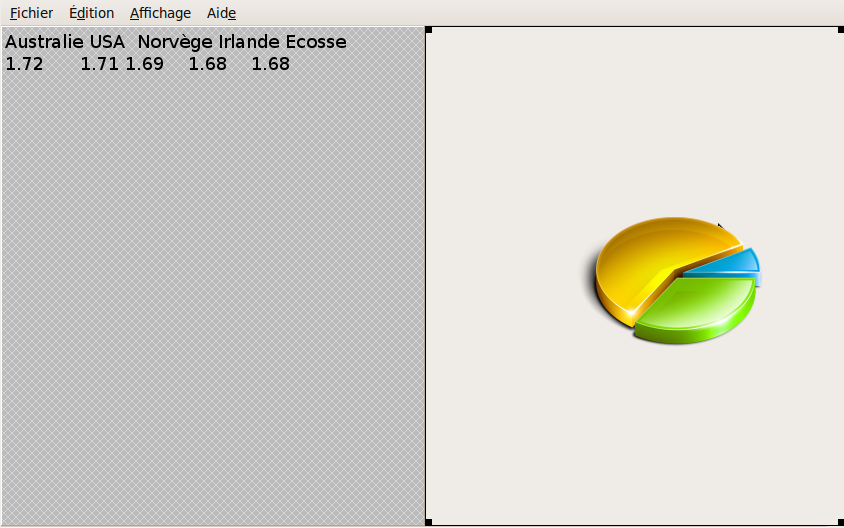
\includegraphics[scale=0.40]{img/soft}
    \caption{Apparence graphique de LoCD}
    \label{fig:apgraph}
  \end{figure}
Pour les utilisateurs peu à l'aise avec l'utilisation des commandes unix, LoCD propose un interface graphique. Bien qu'encore en developpement, cette interface permet de reprendre la plupart des fonctionalités disponibles en lignes de commandes. 
%\clearpage

%%%%%%%%%%%%%%%%%%%%%%%%%%%%%%%%%%%%%%%%%%%%%%%%%%%%%%%%%%%%%%%%%%%%%%%%%

\section{Lancement de l'application graphique}
\label{sec:lancegraph}
Si vous n'avez pas encore installé LoCD sur votre ordinateur, rendez vous à la section \ref{sec:install}. Une fois l'installion complète, il ne reste plus cliquer sur l'executable. Celui ci se trouve à l'emplacement : \verb+/.../LoCD_folder/bin/Locd+. Si un problème à lieu à ce stade, vérifiez que nous avez bien les configurations requises (\ref{sec:conf}). Pour tout autres problèmes \href{mailto:LoCD_assistance@exemple.com}{envoyez nous un mail}.

\section{Utilisation de l'interface graphique}
Voici un bref descriptif des différentes opération proposée par l'interface graphique de LoCD
\subsection{Barre des menus}
Les opérations générales sont listées dans la bare des tâches.
 \paragraph{Fichier}
 \begin{itemize}
\item
Ouvrir : Charger un ficher de données.
\item
Enregistrer : sauvegarder au format «.locd».
\item
Enregistrer sous : préciser le nom de votre sauvegarde.
\item
Exporter : Enregistrer votre diagramme au format de votre choix (pdf ou png).
\item
Quitter : Fermer l'application LoCD.
 \end{itemize} 
 
 \paragraph{Edition}
Ce menu possède le même contenu du menu contextel :
  \begin{figure}[htbp]
    \centering
    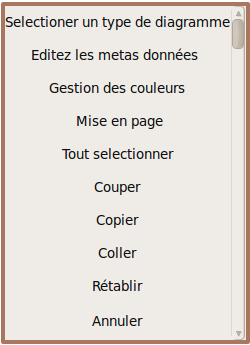
\includegraphics[scale=0.60]{img/menucont}
    \caption{Apparence du menu contextuel}
    \label{fig:menucont}
  \end{figure}

Les opérations : Selectioner un type de diagramme, Editez les metas données, Gestion des couleurs et Mise en page  effectuent les même règlages que ceus décrite dans le chapitre consacré à  l'utilisation par un terminal (\ref{chap:useterm}). Nous vous renvoyons à ce chapitre pour prendre connaissances de ces effets. La seule opération disponible exclusivement dans le menu edition est la rubrique Configuration par défault. Une nouvelle fenêtre s'ouvre et vous propose de régler des différents paramètres (couleurs, mise en page \dots) présents à la figure \ref{fig:dbatons}. 

\chapter{Fichier d'entrée}
\label{chap:fichDonnees}
L'utilisation de LoCD requière en entrée un fichier texte à la sytaxe précise. Ce fichier est composé de deux parties : Méta données et données.
\section{Partie Meta données du fichier d'entrée}
C'est ici que sont définies si besoins les informations décrivant le diagramme. Il est possble d'y préciser 3 sortes d'informations. 
\begin{enumerate}
\item
  Le titre 
\item
  Un sous titre
\item
  Une note
\end{enumerate}
Ces trois donnée doivent être décrite de la manière suivante : 
\begin{enumerate}
\item
  Une ligne par information 
\item
  Une ligne commence par  « > »
\item
  Un des trois mots clefs suivants : \begin{verbatim} TITLE SUBTITLE NOTE \end{verbatim}
\end{enumerate}
Un non respect du format qui va être décrit ci-après soulevera de l'erreur suivante  : 
\begin{figure}[htbp]
  \centering
  
\includegraphics[scale=0.40]{img/eformatfichier}
  \caption{Erreur : format}
  \label{fig:enbdonees}
\end{figure}
Si vous utlisez LoCD avec un terminal, le même texte de l'erreur apparaitra.



\section{Données}
Elles seront renseignées sur deux lignes. La première renseignera les étiquettes des données. Elles seront séparées par un ou des espaces (ou caractères de tabulation). Les valeurs seront sur la ligne suivantes. Les espaces (et\/ou caractères de tabulation) permettent de séparer deux étiquettes ou deux données :
\begin{verbatim}
Etiquette1 Etiquette2     Etiquette3 			Etiquette4
 \end{verbatim} 
 
Toutes les lignes ont une taille d’au maximum 80 colonnes. Dans le cas contraire l'erreur suivante sera relevée : 
\begin{figure}[htbp]
  \centering
  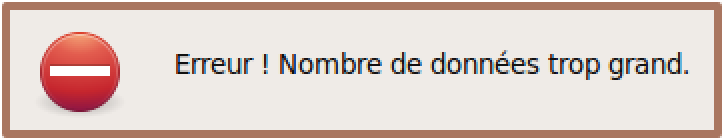
\includegraphics[scale=0.40]{img/enbdonnes}
  \caption{Erreur : nb données}
  \label{fig:enbdonees}
\end{figure}



\section{Exemple de fichier d'entrée}
Pour synthétiser les différents abordés dans ce chapitre voici un exemple de fichier d'entrée valide : 
\begin{verbatim}
  >TITLE: Les plus grands pays du monde pays (~2010)
  >SUBTITLE: En km²
  >Note: La France n'est que 42\up{ème}

  Russie      Canada 	   États-Unis    Chine 	    Brésil 
  17 098 242  9 984 670  9 629 091  	9 596 961  		8 514 877 km2 	
\end{verbatim}
sources \cite{wiki}

\chapter{Fonctionalités}
Nous détaillerons dans cette partie les différentes fonctionalités que propose l'outil. Des exemples illustrés et des \dots  
\section{Histogrammes}
Type de diagramme répendu, l'histogramme fait partie des diagrammes que LoCD peut générer. L'exmple ci-dessus illustre un résultat basique avec la configure par défaut de LoCD soit : 
\begin{itemize}
\item
Une unique couleur : bleu
\item
Absence de titre, sous titre et notes
\item
Représentation 2D
\end{itemize}
Pour changer cette configuration par défault, se référer au chapitre configuration% références !!!!!
\begin{figure}[htbp]
\centering
  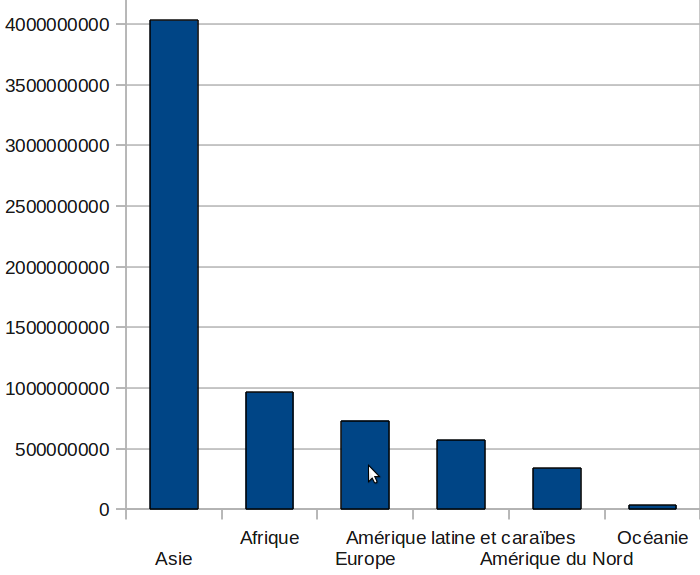
\includegraphics[scale=0.40]{img/diagrammebaton}
  \caption{Histogramme avec les paramètres par défaults}
  \label{fig:dbatons}
\end{figure}
  blah  blah  blah  blah  blah  blah  blah  blah  blah  blah  blah  blah  blah  blah  blah  blah  
\section{Diagrammes circulaires}
LoCD permet la création de diagrammes circulaires similaires  à celui présenté ci-dessous : 
\begin{figure}[htbp]
\centering
  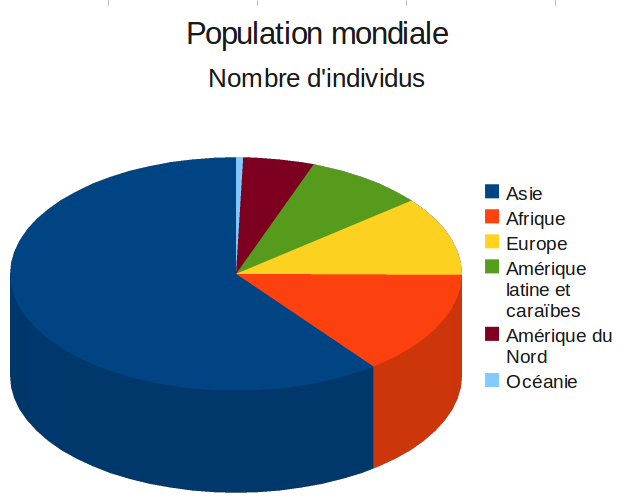
\includegraphics[scale=0.40]{img/diagrammecirculaire}
  \caption{Exemple avec un titre et un sous titre fournis dans les métas données.}
  \label{fig:dcirculaire}
\end{figure}
 blah  blah  blah  blah  blah  blah  blah  blah  blah  blah  blah  blah  blah  blah  blah  blah 
\clearpage
\section{Nuages de points}
\begin{figure}[htbp]
\centering
  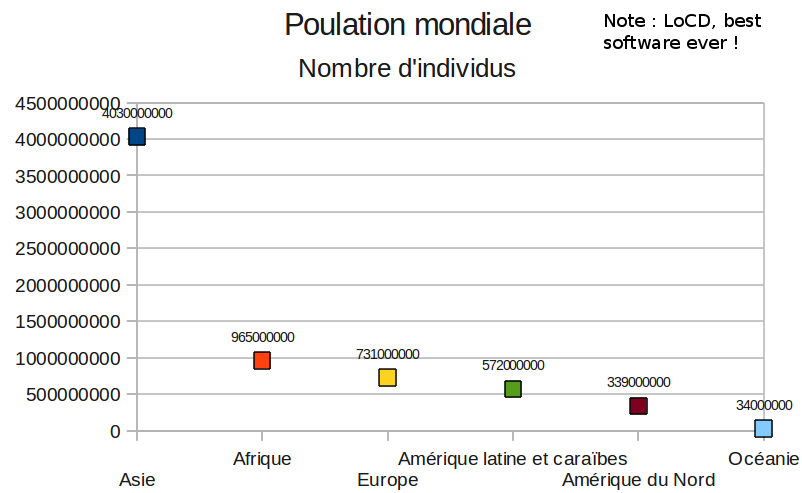
\includegraphics[scale=0.40]{img/diagrammenuages}
  \caption{Nuages de points avec toutes les méta données possible renseignées}
  \label{fig:dnuages}
\end{figure}  
  blah  blah  blah  blah  blah  blah  blah  blah  blah  blah  blah  blah  blah  blah  blah  blah 
  

\chapter{Utilisation console}
 
LoCD peut être utilisé uniquement en ligne de commande. Cette partie demandes des connaissances pré requises sur les commandes unix. En effet seul les fonctionalités de l'outil seront explicitées. La mecanisme des options est similaire à toute autres commandes unix. Pour plus de d'information sur les commandes unix, nous recommandons l'ouvrage suivant : \cite{linux}
%%%%%%%%%%%%%%%%%%%%%%%%%%%%%%%%%%%%%%%%%%%%%%%%%%%%%%%%%%%%%%%%%%%%%%
\section{Utilisation basique}
\label{sec:usebas}
La simple commande suivante générera un pdf avec d'un histogrammes avec les paramètres par défaut : % rajouter ref!!!!
\begin{verbatim}LoCD inputfile.txt\end{verbatim}Les choix du type de diagramme est possible grâce à l'option \verb+-t+ (ou \verb+--type+ ) suivit de : 
\begin{itemize}
\item
\verb+circulaire+ pour un diagramme circulaire.
\item
\verb+histogramme+ pour un histogramme.
\item
\verb+nuage+ pour un diagramme en nuage de points.
\end{itemize}
%%%%%%%%%%%%%%%%%%%%%%%%%%%%%%%%%%%%%%%%%%%%%%%%%%%%%%%%%%%%%%%%%%%%%%%%%%%%%%%%%%%%%%%%%%
\section{Gestion des méta données}
Une option pour chacune des méta données disponible (cf : ~\ref{chap:fichDonnees}) est définie :
\begin{itemize}
\item
\verb+-t+ ou \verb+--title+ pour afficher le titre.
\item
\verb+-s+ ou \verb+--subtitle+ pour afficher le sous titre.
\item
\verb+-n+ ou \verb+--note+ pour afficher le sous titre.
\end{itemize}
Si une de ces options est renseignée, il est possible de rajouter une valeur pour le paramêtre concerné. Par exemple : 
\begin{verbatim}
LoCD --title "Mon titre de diagramme" --subtitle "le sous" titre"
\end{verbatim} 
Dans le cas où l'une de ces options serait rajoutée ; et que aucune valeur ne lui est attribuée (en ligne de commande ou dans le fichier d'entrée) ; un avertissement apparaîtra à l'execution. Le diagramme n'aura pas de sous titre.\label{err:optmissing} % rajouter une ref!!!
%%%%%%%%%%%%%%%%%%%%%%%%%%%%%%%%%%%%%%%%%%%%%%%%%%%%%%%%%%%%%%%%%%%%%%%%%%%%%%%%%%%%%%%%%%

\section{Mise en forme reglages divers}
Le diagramme obtenu dans le cas d'une utilisation basique (~\ref{sec:usebas}) est stocké dans le dossier courant sous le nom de \verb+new_file.pdf+ et à les caractéristiques graphiques suivantes illustrée dans la figure :  ~\ref{fig:dbatons}.\\ Le changement du nom de ficher de sortie peut être modifier en rajoutant l'option \verb+-f outfilename+ ou dans sa version longue \verb+--filename+. 
\subsection{Couleurs}
\label{subsec:couleurs}
L'option \verb+-c+ (\verb+--couleur+) permet d'éditer la couleur de chaque données. Dans cette version LoCD propose une palette de 6 couleurs :
\begin{itemize}
\item
orange
\item
rouge
\item
vert
\item
bleu
\item
bleu ciel
\item
violet
\end{itemize}
Deux méthodes sont possibles :
\begin{enumerate}
\item
Faire suivre l'option d'un nom de couleur (listées ci-dessus). Le diagramme aura alors cette unique couleur.
\item
Faire suivre l'option du nom de la donnée puis d'un «couple» nom\_donnee:couleur séparé par le caractère \verb+:+. Une ou toutes les données peuvent être ainsi précisées. Dans tout autre cas, la couleur par défaut sera appliquée.
\end{enumerate}   
\subsection{Mise en page}
\label{subsec:misepage}
Dans la configuration par défault. Le diagramme est centrée dans une page de format A4 («au centre»). Le titre et le sous titre sont placés au dessus du diagramme (au nord»). La note elle, est placée à droite de des titres («nord est»). La figure \ref{fig:dnuages} est l'illustration de cette mise en page par défaut.
 


% Pour finir l'interligne de 1,5
\listoffigures
\printindex

\appendix
%\bibliographystyle{AB_bib}
\bibliographystyle{alpha}
\bibliography{/home/alain/workspace/Latex/manuel/biblio.bib}

\end{document}
